\section{Experiments}
In an effort to carry out a proper experiment, we applied a variety of methods to our data.
From Natural language processing to non-linear models, the following subsection describes the motivation behind the choices we made in this department and outlines our performance predictions.

We experimented with two techniques for our baseline models, excluding our linguistic features of course, because one of the primary questions we aim to answer in this paper is whether the added linguistic features we extracted using the natural language processing pipeline improve the classification of disaster tweets compared to classic derivable features.

\subsection{First attempt: Logistic regression}

For our first baseline model, we wanted a simple and statistical approach.
Logistic regression serves our purpose nicely, taking multiple numerical features and outputting a binary response probability.
In this specific case we employ this model with 2 feature extraction methods: Bag of words and Term frequency-inverse document frequency (TF-IDF).
Bag of words is a simple text feature extraction method, it builds a vocabulary of unique words it encounters throughout the input and keeps a measure of their occurrences.
TF-IDF takes the concept a step further by multiplying the measure (term frequency) by the term's inverse document frequency: in our setting this translates to multiplying the frequency of a word in a tweet by a measure of how rare or common it is in the corpus (set) of tweets.

Term frequency Inverse document frequency in our setting is defined as:

$$
\text{TFIDF} = \frac{\text{number of occurrences of a term}}{\text{total number of words in the tweet}} \log{\Big( \frac{\text{total number of tweets}}{\text{number of tweets containing the term}} \Big)}
$$

The logistic regression model then uses a logit function to estimate probabilities. This function is defined as:

$$
F(x) = \frac{1}{1-e^{-x}}
$$

where

$$x = w_0 + \sum_{k=1}{n} w_k \cdot x_{k}$$

$w_k$ are the regression coefficients of the model and $x_k$ are the features.
The results of this model can be depicted in a confusion matrix, as shown in \autoref{fig:confusion-matrix} in the appendix.
These results are particularly bad, considering we have a large amount of false positives, meaning that a large number of non disaster related tweets were classified as disaster, if we consider cost imbalance, this is not as bad as having the opposite scenario.
We can conclude on this basis that this regression model is indeed a bit brave (classifies most data points as positive).

\subsection{Experimental setup: The Pipeline}

To enable several experiments using different classification methods, some sort of pipeline needs to be established.
To turn our data set in training data points, we assemble together a 5 component pipeline.

The Data preprocessing elaborated in previous sections is the first part of our pipeline,this section handles data cleaning and exploration, i.e generating more features.
Consequently, the training data points become more and more complex throughout the pipeline, both in terms of data type and format.
At the end of the process, the training data contains numerical, textual and categorical labeled data.
Therefore, the second part of the pipeline is a column transformer from the Scikit-learn library which is responsible for serializing all kinds of extracted features from every column into scalar values.
Then, the third part of the pipeline is a scalar which normalises these scalar values to the same range in order to prevent bias.

The experimental part is the fourth part, which is regarded as a slot where different classification methods are “plugged in” to produce predictions.
Finally, the last part of the pipeline is the evaluation of the predictions, for this matter we used cross-validation with 5 stratified folds for all experiments, furthermore the loss measurement is based on the mean square error (MSE) of the classifiers.
We rely on this measure as a primary means to compare classifiers and test our hypothesis
In an effort to carry out a proper experiment, we applied a variety of methods to our data.
From Natural language processing to non-linear models, the following subsection describes the motivation behind the choices we made in this department.and outlines our performance predictions.

We experimented with two techniques for our baseline models excluding our linguistic features to help us answer the research question.

\subsection{Baseline method: Linear SVC with derivable features (non-NLP)}
The method that we used for our baseline is Support Vector Classifier (SVC), a statistical model built using support vector machines.
The goal behind SVM is to find the decision surface that maximizes the margin between the data points of the two classes (disaster related or not in this case).
This decision surface is best illustrated through the following figure from \cite{4}:

\begin{figure}[h]
  \centering
  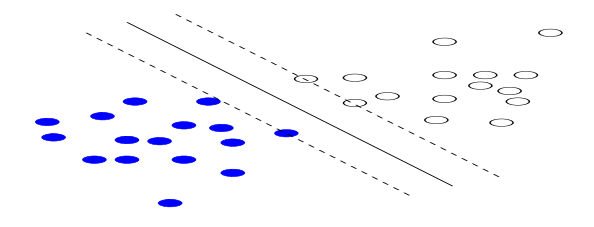
\includegraphics[scale=0.5]{decision-surface.png}
  \caption{A decision line (solid) and a margin (distance between dashed lines), both represent the decision surface.}
  \label{fig:decision-surface}
\end{figure}

Mathematically, this decision surface (for linearly separable data) can be written as a hyperplane \cite{4} where the vector x is a data point we want to classify whereas w and b are learned from the training set :

$$vec(w_i) \cdot vec(x_i) - b = 0$$

Let $y_i$ be the classification of a data point $vec(x_i)$. If it evaluates to +1 for positive and -1 for negative, the SVM optimization problem can be simply written as the following two inequalities:

$$
\begin{cases}
  vec(w_i) \cdot vec(x_i) - b \geq +1, &\text{for } y_i = +1 \\
  vec(w_i) \cdot vec(x_i) -b \leq -1, &\text{for } y_i = -1
\end{cases}
$$


One way to motivate this choice for our task would be to showcase comparative studies involving SVM and text classification, and indeed we do provide a few studies showing that Support Vector Machines can provide state-of-the-art performance in text classification tasks \cite{3,4}.
We will show later that our Linear variant of SVC however loses horsepower against its non linear counterparts, this is partly due to our added NLP features breaking the linear separability property of our dataset.
More on this in the next section.

\subsubsection{Feature Pre-elimination}

Before deploying the linear SVC method, we were eager to evaluate the usefulness of some features.
To this end, we set up a quick comparison (not using our full pipeline) comparing the results of using the id feature or not.
As expected, The metrics shown in \autoref{fig:feature-pre-elim-metrics} demonstrate that the id feature has a negative impact on the prediction, we decided to omit it for later stages.

\subsubsection{Exploiting Feature Space with Kernel Tricks}

Before we proceed with adding more and more features, we need to uncover some properties of the training data.
In this subsection we employ a variety of kernels for our SVC model (using kernel trick), furthermore based on the results we will be able to make assumptions about the shape and condition of the data.


First, an assumption is made that the feature space before extracting more features should be linearly separable.
To prove this, several experiments using SVC with 3 kernel types, rbf \cite{x1}, polynomial and sigmoid, are conducted.
It turns out, based on the results shown in \autoref{fig:rbf-kernel-tricks} and \autoref{fig:poly-kernel-tricks}, this is indeed the case that the linear kernel outperforms other 2 non-linear kernels using only basic features serialized from the original dataset.
Our assumption holds so far.
Furthermore, based on the training set accuracy, the SVC with \verb|poly| kernel seems to have overfitted and the overall standard deviation of the predictions is quite high.

\subsection{Non-baseline methods: (NLP) Entity-related Features}

Without using any NLP-related features, the performance of the prediction is about 50 - 60\% accuracy if taking the variations into account. The current scores are by no means close to yielding a useful model. However, since the feature space is still rather naïve, exploring more features with natural language processing seems promising.

To build our NLP component, we used one of the best performing NLP libraries at the moment, SpaCy \cite{x2,x3}. Since concrete entities are reflected through the tweets, we will use these as central features and derive the other features from them. Following this protocol, we end up with 5 features : the entities themselves,  the labels/types of the entities, the words dependent on the entities (Part of speech), the positions of the entities in a sentence (Part of speech) and the derived words of the entities.

\subsubsection{SVC - The Second Try}
Having the previous performances on hand, more experiments were undertaken using SVC.
Similar to the previous method, an experiment using the linear kernel was first conducted.
Then, experiments using non-linear kernels are followed.
The results of experiments in question are summarised in \autoref{fig:linear-kernel-svc}, \autoref{fig:rbf-kernel-svc},
\autoref{fig:poly-kernel-svc}, and \autoref{fig:sigmoid-kernel-svc} in the appendix.


As a corollary, the performances of most of the non-linear kernels have surpassed that of the linear kernel.
We, therefore, conclude that, after adding the 5 entity-related features, the feature space is no longer linearly separable.
Most importantly, the scores of the predictions have been improved a lot which gives away the possibility of having further improvement by adding more relevant features.
In addition, the prediction produced by the polynomial kernel is exceptionally bad, therefore we decided to omit it from the next experiment.

\subsubsection{Classification ensemble with Adaboost}

Although the performance got improved by adding those entity features, the bias of the results remains huge as the accuracy is still below 65\%.
Thus, ensemble methods with boosting \cite{x4} in turn become the next attempt with the purpose of reducing bias and improving accuracy.
An adaboost classifier is then plugged into the pipeline.
The results of this experiment are illustrated in \autoref{fig:adaboost} in the appendix.

Surprisingly, the result is not good at all as it barely reaches the same accuracy as that of the SVC with the polynomial kernel.
Therefore, this method was discarded at this phase.

\subsubsection{Bagging with Random Trees}
Decision trees are by nature one of the most intuitive machine learning algorithms humans ever designed, most people have at some point employed this line of reasoning while trying to make a decision, hence its grand popularity in classification.
Let’s deviate slightly from the statistical math heavy illustrations and turn to a simple example that shows how this decision trees function in
\autoref{fig:decision-tree}:

\begin{figure}[h]
  \centering
  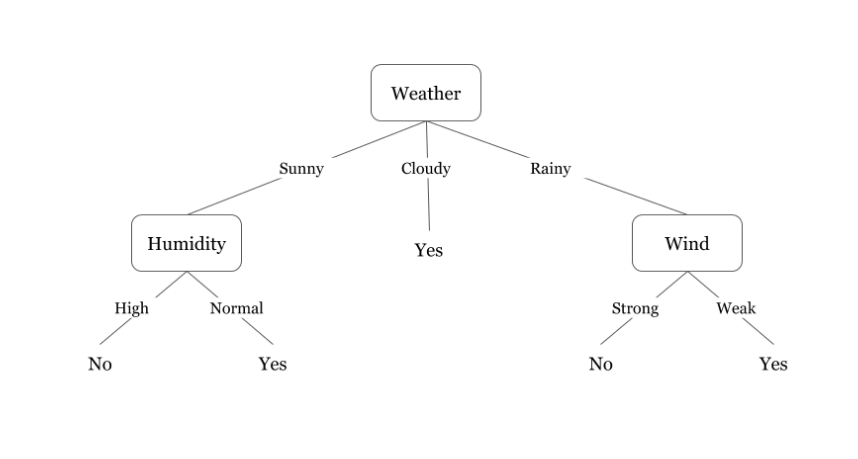
\includegraphics[scale=0.3]{decision-tree.png}
  \caption{Graphical representation of a decision tree on the problem: Should we play badminton or not based on weather conditions}
  \label{fig:decision-tree}
\end{figure}

As you can see, a tree is a collection of if-then conditional rules to reach a binary decision “yes-no” (we only illustrated binary classification
for our purpose, but it can also classify labels) \cite{6}.

For our purpose, we are using decision trees in an ensemble, more accurately, a random forest, one of the most famous bagging methods, particularly famous for feature selection, a deciding factor in our decision to conduct experiments using this method.
This model works by spawning multiple decision trees each with a random subset of features and training data, it then pools the predictions together
and takes the average, take this as a multitude of humans making predictions about a specific matter, if the matter is hardly predictable, pooling and
averaging predictions can help reach a more precise result \cite{10}.
The prediction results using the Random Forest classifier with our current limited set of 9 features are demonstrated in figures
\autoref{fig:20-trees}, \autoref{fig:200-trees}, and \autoref{fig:500-trees} in the appendix.

As the results show in the tables, using the random forest method improves the accuracy to about 68\% which is the most promising result we have so far.
However, when looking at the variance and the training set accuracy, it shows us that the model is prone to overfitting, especially when the number of bagged trees reaches about 500, and the accuracy starts dropping.
For this reason, we decided in the following experiments, that a maximum depth for each considered decision tree should be set.


\subsection{Feature Post-processing: selecting the right features}
At this stage, lots of features have been extracted and utilised.
As elaborated in the data preprocessing section, both quality and quantity of the features play a vital role in the classification process.
Therefore, we decided to conduct feature post-processing before adding more features.

\subsubsection{Imputation and Feature Importance}

In the conducted experiments, missing values are filled by dummy values or labels like ``missing'' or ``unknown''.
However, as discussed in the previous section, missing keywords should be replaced by the mode of each class, the real disaster class and the fake disaster ones.
Thus, a simple imputation by replacing those dummy fillers with corresponding mode values is implemented.
However, surprisingly, the prediction accuracy compared to before shows no noticeable improvement.
This is shown in \autoref{fig:replace-keyword-svc} in the appendix.

Additionally, we examine the feature importance by looking into the top-10 features that are selected by the random forest classifier.
In the appendix, \autoref{fig:top10-features-without-text} shows the top-10 features without text data and  \autoref{fig:important-features} illustrates the important features in the text data.
After analysis, each elected feature category plays an important role in the classification process.

\subsubsection{Polynomial Feature Extension}

Without using more NLP features, the simplest way to achieve massive features is to create new features based on existing features.
One of the approaches is to generate polynomial and interaction features the way resembles that of the polynomial kernel trick.
To this end, a polynomial feature generator from Scikit-learn library is inserted into the middle of the pipeline.

Originally, 38278 features including all text data have been used in previous experiments.
After inserting a polynomial order-two feature generator, the number of features of each data point is extended to 767869266 (about 770 million).
However, when feeding this amount of features into the random forest (our current best model) the training process could not be accomplished after 5
hours of training in the supercomputer DAS5 \cite{x5}, we thus decided to go with the SVC model with the rbf kernel.
The result is shown in \autoref{fig:svc-rbf-kernel} in the appendix.

To our surprise, the performance did not improve as expected.
Therefore, we conclude that more features do help in terms of the classification only if the added features are relevant and carefully selected.

\subsection{Final Model Selection: Using full NLP feature set}
Finally, after several experiments, the ideal computational models that fit into our scenario are narrowed down to Random Forest.
At this final stage, we will make use of all NLP features described in \autoref{tab:feature-stats} together with the 5 entity-related features to evaluate the models.

\subsubsection{The Black-Box - Neural Net }
Before our final run of the Random Forest model, it would be really interesting to see how all the features perform in a black-box neural network.
We thus chose the most straightforward NN method, Multi-layer Perceptron (MLP) classifier \cite{x6} to see whether there would be any promising results.
Again we provide a usability case study \cite{8} on why this model would be a promising choice. The results of this experiment are shown in \autoref{fig:mlp-all-features} and \autoref{fig:mlp-all-features-2000} in the appendix.

As illustrated in the resulting tables, there is indeed small performance gain by enlarging the neural network.
However, considering the exponential increase of the training and evaluation time, we have to give up this method and stick with the Random Forest model.

\subsubsection{Tuning Hyperparameters of the final model - Random Forest}
Since examining the best number of trees and the maximum number considered for each tree are known to be the most time-consuming part, we, therefore,
make tuning of these two parameters a stand-alone process by drawing the out-of-bag (OOB) error curve \cite{x7} in order to see the convergence region so that we can to narrow down the range of the parameters and in turn shrink the random search grid.

\begin{figure}[h]
  \centering
  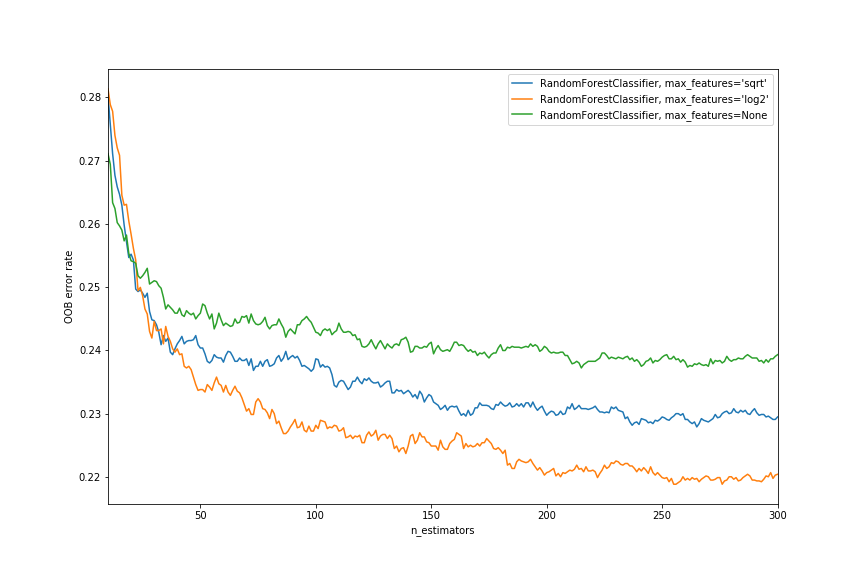
\includegraphics[scale=0.5]{curve.png}
  \caption{}
  \label{fig:curve}
\end{figure}


By setting up 3 pipelines with different \verb|max_features| parameters, we continually tune their \verb|n_estimators| parameters which resulted in
the OOB error curve showing in \autoref{fig:curve} in the appendix.

Based on the OOB error curve that we have, the best parameter for \verb|max_features| would be \verb|sqrt|.
For the \verb|n_estimation| parameter, there is a clear convergence around 250.
Thus, we finally shrink down the parameter distribution into the following,

\begin{verbatim}
random_distro ={
     'bootstrap': [True, False],
     'max_depth': [10, 20, 30, 40, 50, 60, 70, 80, 90, 100, None],
     'max_features': ['sqrt'],
     'min_samples_leaf': [1, 2, 4, 6, 8],
     'min_samples_split': [2, 5, 10],
     'n_estimators': [220, 250, 270]
}
\end{verbatim}


Further, a randomized search on hyperparameters is conducted using the Scikit-Learn library.
The result of the random search is shown in \autoref{fig:base-random} in the appendix.

\begin{verbatim}
{'n_estimators': 250,
 'min_samples_split': 6,
 'min_samples_leaf': 4,
 'max_features': 'sqrt',
 'max_depth': 80,
bootstrap': True}
\end{verbatim}

By comparing the base model of the random forest whose performance is shown in \autoref{fig:random-hyper} in the appendix, an improvement on the cross-validation accuracy of about 3\% can be concluded and, perhaps most importantly, according to the training set accuracy, the tuned model less prone to be overfitting.
